\section{Monitoring Wireless Devices}\label{sec:monitoring} 
When monitoring wireless devices in indoor spaces, a set of obstacles are presented. Some of the popular techniques used in outdoor environments prove themselves obsolete or severely hindered when applied in an indoor environment. This can be seen when working with the Global Positioning System(GPS) technology, as obstacles such as walls, roofs and floors will disrupt the signals received from satellites, leading to large imprecisions in the position measurement \cite{gps_indoor}. As a consequence we need to explore specialized methods for determining positions in indoor spaces.

In this section we will explore different approaches for indoor positioning and monitoring mobile devices, and examine systems using these.

\subsection{Tracking Approach}\label{sec:tracking_approach}
WI-FI, Bluetooth and Radio-Frequency Identification (RFID) are amongst the most popular technologies used for indoor positioning. When using these technologies there are multiple approaches for determining a users position. In this section we will examine some of these approaches.

Tracking approaches are typically mapped into four categories \cite{tracking_approaches}
\begin{itemize}
\item Cell of Origin
\item Distance
\item Angle of Arrival
\item Location Patterning
\end{itemize}
Despite the partitioning, many advanced approaches combine categories to increase the location accuracy. We will take a look at an approach from each category.

\subsubsection*{Cell of Origin}
Approaches categorized under cell of origin are among the simplest techniques for positioning. These approaches aim to position mobile devices in cells, either defined by the reach of access points, or defined by rooms in a building.
The latter approach can utilise RFID to create checkpoints throughout a building. These checkpoint are placed in room entrances and consist of a RFID scanner, such that devices with a RFID tag are registered as they pass by the scanner \cite{indoor_bin}. 
This approach can be used to track the RFID tags, as each tag contains a unique ID, which is combined with the RFID scanners ID and a time-stamp. By analysing the most recent entry, the system will know which room the tag is located in \cite{RFIDjournal}.

The approaches in this category require auxiliary hardware to set up the checkpoints, and is in addition to this limited to only register movement at these checkpoints. By analysing the collected data on the host system it is possible to track a device. Thereby it can be derived if a device has entered or exited the room. It is, however, not possible to know where in the room a device is, which makes it difficult to track someone if a room is of substantial size or the building lacks RFID scanners \cite{RFIDjournal}.

\subsubsection*{Distance}
Approaches in the distance category measures the proximity of a device and use this information to calculate a position, much in the same way it is done by GPS.
Triangulation works by using three or more access-points to receive the signal from a device. The position of the access-points is known to the system, and by calculating euclidean vectors from each access-point to the device, based on the Received Signal Strength Indication(RSSI), the position can be found \cite{Triangulation}. The RSSI can be used to measure proximity, using the fact that signal strength decays over distance. Naturally, the decay will be greater in a closed environment with obstacles causing signal disruptions, and as such signal loss models have been developed for indoor environments. 
\Cref{fig:triangulation} shows a simple model of how triangulation works. In the centre of each circle is a set of coordinates encoding the position of the access-point. The circle indicates the proximity of the device based on the signal strength. With the use of three access-points we can determine the position of the device, by calculating the position of the intersection of the proximities.
\begin{figure}[ht]
	\begin{center}
		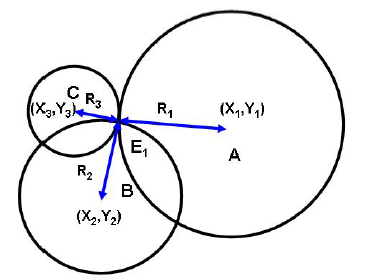
\includegraphics[scale=1]{graphics/triangulation.png}
		\caption{Triangulation \cite{Triangulation}}
		\label{fig:triangulation}
	\end{center}
\end{figure}

\subsubsection*{Angle of Arrival}
This category consists of approaches where the angle of the received signal is measured. The angle can be obtained by either having several antennas or being able to rotate a single antenna to find the direction at which the RSSI is strongest. With multiple angles of arrival it is possible to calculate a position based on the intersection of the euclidean vectors going through the antennas. \sfx{Same source as other places, need to cite though}

\subsubsection*{Location Patterning}
The location patterning category sets out to measure the connectivity patterns for a set of locations. The most common approach for this category is called WI-FI Fingerprinting. This method has an intial calibration phase, where the RSSI pattern for each point of interest is measured and stored in the system. When the signal strength from a device is received, it is then compared to the previously measured RSSI patterns. The point of interest with the most similar pattern is determined to be the position of the device. This means that a system using fingerprinting can not determine the exact position of a device, but rather calculates a probability that the device is located at a given point of interest \cite{fingerprint1}.

\subsection{Evaluation dimensions}
When evaluating indoor location services there are three dimensions that we can evaluate quality on: location precision, refresh rate and system latency. Location precision tells us about the location precision that the system affords. Refresh rate is the rate at which the location is updated, and as such how closely the most recent data is related to real-time data. System latency is a dimension describing the time it takes to perform the positioning calculations \cite{dimensions}. These dimensions are not standardized, but we view them as reasonable initial parameters for comparing the systems.

The three dimensions are in no way constant for a system. For most systems, the hardware has a large influence on the dimensions. For instance, location precision for Triangulation is severely diminished if the environment lacks access points. Refresh rate depends on how often mobile devices communicate with the network and system latency can be impacted by a large amount of noise on the WI-FI channels. \Cref{tab:evaluating_approaches} shows the influences for the four tracking approach categories for each evaluation dimension. As the table shows, it is primarily the location precision that has various dependencies across the approaches. The refresh rate will in most cases depend on the interval at which the device communicates, while the system latency entirely depends on the software, hardware and communication protocols used.

\begin{table}[]
\centering
\begin{tabular}{|l|p{4cm}|p{4cm}|p{3.5cm}|}
\hline
                    & Location Precision                 & Refresh Rate             & System Latency    \\ \hline
Cell of Origin      & Depends on cell size				 & On checkpoint register   & Depends on system \\ \hline
Distance            & Depends on amount of access points & When device communicates & Depends on system \\ \hline
Angle of Arrival    & Depends on amount of antennas      & When device communicates & Depends on system \\ \hline
Location Patterning & Depends on calibration phase       & When device communicates & Depends on system \\ \hline
\end{tabular}
\caption{Evaluation dimension in relation to the four tracking approaches}
\label{tab:evaluating_approaches}
\end{table}


\subsection{Technologies}
In this section we examine some systems using different tracking approaches that aSTEP can use to integrate indoor positioning.

Zonith Indoor Positioning System is a system that uses the cell of origin approach. As mentioned in \cref{sec:tracking_approach}, this technique requires auxiliary hardware. Zonith offers Bluetooth Beacons, which serve as checkpoint nodes, and allow for any device with Bluetooth to be discovered and tracked \cite{zonith}. Because of the nature of the approach we expect the location precision to be excellent at the moment the device is registered, and the quality of the data decays as it ages. However, the most recent registration of a device is an approximation of its location, at best it tells us what room the device is in.

Redpin is an open source indoor positioning system that uses location patterning. The system requires a calibration phase, where the connectivity fingerprint of different key locations is measured. A user's location is calculated on request, and, with enough fingerprint measurements, the system will be able to provide the user with at least room-level accuracy \cite{redpin}. Location precision is as such dependent on the calibration phase, but is expected to be better than a cell of origin approach. 

Google have also developed their own positioning system. They have made indoor navigation and tracking possible trough their Indoor Maps project \cite{IPSoverGPS}, which lets users map a building by uploading a floor plan of said building. After the floor plan has been accepted, the system will request information about the location of the WI-FI access points in the building \cite{googleindoormaps}. A user can then see their own location on Google maps at any time. Google have been very secretive in regards to what tracking approaches they use, as such it is difficult to evaluate the technology.

Cisco have developed a location-aware wireless network system, Cisco Mobility Services Engine (MSE), which utilises WI-FI triangulation \cite{CiscoTri}. MSE makes it possible to track the location of up to 25000\sfx{double check this number} network devices at once, regardless of whether the devices are connected to the network. Using the RSSI data from the access points, the MSE controller calculates distance and compares time of arrival to perform a triangulation and obtain a position \cite{ciscoMSE}.
The building is modelled by the use of an outline of the floor plan. The image is converted to a coordinate system that is placed on top of the model, which is then supplied with the positions of the static access points in the building. With this information it is possible to get the relative position of any device in relation to the origin of the coordinate system. It is these relative positions that are used to track wireless devices. MSE also has the capability of calculating geographic coordinates.
Cisco claim to have a location precision of less than 1 meter, refresh rate of 10-120 updates per minute and a system latency of 2-4 seconds \cite{dimensions}. 

\subsection{Choice of Technology}\label{subsec:cisco}
We have presented four technologies using different tracking approaches. We impose two requirements for the technology. First, we largely prefer a system with an accurate location precision. In practice this means being able to position people within rooms, as indoor environments can differ greatly in room size. For instance, an airport is difficult to partition into rooms, as it normally exhibits very large open spaces. Secondly, we wish to harvest as much data, in terms of positions, as possible. This allows for predictions on crowd movements, path-finding to circumvent crowded areas and analysing typical movements in a building. 

\Cref{tab:evaluating_approaches} displayed that the location precision for the Cell of Origin approach depends on the cell size. The precision will at best be within a cell, which in the case of the Zonith Indoor Positioning System is equivalent to a room. Our first requirement therefore excludes the Zonith Indoor Positioning System. To accommodate the second requirement, we examine the obtainable data from the systems. Redpin affords the possibility to request the position of a single device. Given that it is open source, it will be possible to alter the system in such a way that all devices on the network is provided. Google Indoor Maps only allows requesting a single user. Cisco MSE has the functionality to provide a list of devices registered along with their most recent position.

There are several arguments pointing towards Cisco MSE rather than Redpin. First and foremost, Cisco MSE is in comparison a lot more convenient, as it already affords the desired functionality and requires substantially less set-up time. Secondly, the amount of documentation for Cisco MSE far outweighs what little documentation there is for Redpin. Cisco MSE is a commercial system, and is therefore updated regularly. As of 7/3/2016, Redpin had its most recent update in May 2013. Lastly, Redpin only claims to be able to position devices at room-level precision, while Cisco claims to position devices within rooms. As a consequence of these arguments we chose to integrate MSE for the indoor positioning system for aStep.

Aalborg University uses the standard version of MSE to position wireless devices across all their campuses. We plan on using the data available from this system as mock data for the aSTEP project.